\documentclass[review]{elsarticle}

\usepackage{lineno,hyperref}
\usepackage{subcaption}
\usepackage{siunitx}
\sisetup{group-separator = {,}}
\usepackage{booktabs}
\usepackage{graphicx}
\usepackage{adjustbox}
\usepackage{appendix}
\usepackage{amsmath} 
\usepackage{scrextend}
\usepackage[hang,flushmargin]{footmisc} 
\usepackage{xcolor}
\usepackage{float}
\usepackage{array,multirow}
\usepackage{hyperref}
\usepackage{setspace}
\usepackage{stmaryrd}
\usepackage{enumitem}
\usepackage{rotating}
\usepackage{adjustbox}
\usepackage{array}
\usepackage{booktabs}
\usepackage{xcolor,colortbl}
\usepackage{amsmath} 
\usepackage{amsfonts} 
\usepackage{amssymb}
\usepackage{makecell}
\usepackage{amsmath}
\usepackage{nicefrac}
\usepackage{todonotes}
\usepackage{multirow}
\modulolinenumbers[1]
\usepackage{lineno}
\usepackage{tikz}
\usepackage{cleveref}
\usepackage{accents} 
\usepackage{arydshln}
\usepackage[T1]{fontenc}
\usepackage{pifont}
\linenumbers

% \usepackage[final]{changes}
\usepackage[markup=underlined]{changes}

\usepackage[ruled,vlined,linesnumbered,lined,boxed,commentsnumbered]{algorithm2e}
\newcommand\mycommfont[1]{\footnotesize\ttfamily\textcolor{blue}{#1}}
\SetCommentSty{mycommfont}
\newcommand{\BREAK}{\STATE \algorithmicbreak}
\modulolinenumbers[1]
\setlength{\parindent}{0em}
\journal{Energy}
\bibliographystyle{elsarticle-num}

\begin{document}
\begin{frontmatter}

\title{Shrinking together and pulling apart: insights from a national gas grid with declining natural gas demand and increasing domestic renewable gas generation by 2040}

\author[1,2]{Sebastian Zwickl-Bernhard\corref{cor1}}
\ead{zwickl@eeg.tuwien.ac.at}
\author[3]{Aria Rodgarkia-Dara}
\author[3]{Christoph Gatzen}
\author[3]{Lino Sonnen}
\author[3]{Anna Lane}
\author[1]{Marcus Otti}
\author[1]{Antonia Golab}
\author[1,2]{Hans Auer}
\cortext[cor1]{Corresponding author}
\address[1]{Energy Economics Group (EEG), Technische Universität Wien, Gusshausstrasse 25-29/E370-3, 1040 Wien, Austria}
\address[2]{Industrial Economics and Technology Management, Norwegian University of Science and Technology, Gløshaugen, Alfred Getz vei 3, Trondheim, 7491, Norway}
\address[3]{Frontier Economics Limited, Im Zollhafen 24, 50678 Köln, Deutschland}

\begin{abstract}
	This paper studies the development of the Austrian gas grid by 2040 under different decarbonization scenarios, ranging from electrifying most energy services to importing large amounts of renewable methane. The Austrian gas grid serves as a case study representative for those gas grids confronted with a drop in natural gas demand and an increase in domestic renewable gas generation in the future. A mixed-integer optimization model with a focus on the detailed representation of the existing grid (gas grid levels, pipeline capacity, route, and age) is used to determine the cost-optimal trade-off decision between expected low-utilized gas pipelines and an off-grid supply alternative (e.g., trucking and on-site gas storage) in a decarbonized Austrian and European energy system. Based on the required gas grid 2040 and its annual grid costs, estimates for tariffs of end customers are given. The paper's main conclusion is that the domestic distributed renewable gas generation uptake will be associated with the need for an area-wide gas grid, but one that will be significantly less utilized.
\end{abstract}

\begin{keyword}
	Gas grid; natural gas demand; domestic renewable gas generation; 2040

\end{keyword}
\end{frontmatter}

\newpage
\section*{Nomenclature}
\begin{center}
	\renewcommand{\arraystretch}{1.0}
	\centering
	\small
	\begin{tabular}{lm{8cm}r}
		Type & Description & Unit\\
		\hline
		Set and index & & \\
		\hline
		{$p \in \mathcal{P}=\{1,\ldots,P\}$} & Pipeline for gas transport, index by $p$\\
		{$n \in \mathcal{N}=\{1,\ldots,N\}$} & Node of the gas grid, index by $n$\\
		{$l \in \mathcal{L}=\{1,\ldots,L\}$} & Level of pressure in the gas grid, index by $l$\\
		{$y \in \mathcal{Y}=\{1,\ldots,Y\}$} & Years, index by $y$\\
		{$m \in \mathcal{M}=\{1,\ldots,M\}$} & Months, index by $m$\\
		\hline
		\multicolumn{2}{l}{Decision variables (selected)}\\
		\hline
		{$Capex$} & Capital cost of pipelines in the gas grid & \SI{}{EUR}\\
		{$Opex$} & Operational cost of pipelines in the gas grid & \SI{}{EUR}\\
		{$CoAS$} & Cost of an alternative off-grid gas supply & \SI{}{EUR}\\
		{$\gamma_{p,l,y}$} & Transport capacity of pipeline $p$ at $l$ in $y$& \SI{}{GW}\\
		{$\sigma_{p,l,y}$} & Decommissioning decision of pipeline $p$ at $l$ in $y$ (binary)& -\\
		{$q^{fed, local}_{n, l, y, m}$} & Local gas generation injected into the gas grid at $n$ and $l$ in $y$ and $m$& \SI{}{Year}\\
		\hline
		\multicolumn{2}{l}{Relevant parameters}\\
		\hline
		{$\gamma^{pre}_{p,l,y}$} & Existing transport capacity of pipeline $p$ at $l$ in $y$ & \SI{}{MW}, \SI{}{GW}\\
		{$y^{inv}_{p,l}$} & Year a pipeline $p$ at $l$ reaches its technical lifetime & \SI{}{Year}\\
		
		\hline
	\end{tabular}
\end{center}
\newpage

\section{Introduction}
For decades in Europe, the optimal method of distributing natural gas to end customers, regardless of their varying demand scales (ranging from industrial facilities to individual households), has been through gas pipelines and gas grids \cite{rajnauth2008gas}. The first of two reasons for this is that natural gas has been a cheap energy source due to its virtually unlimited availability in Europe through imports, mainly from neighboring regions \cite{bilgin2009geopolitics}, with the second reason allowing large quantities of natural gas to provide various energy services, being that transporting natural gas through pipelines has been technically efficient and economically cheap over short and long distances \cite{thomas2003review}. This paper aims, among other things, to analyze how these gas grid costs for end customers could develop during decarbonizing energy systems in the future. It is seen that both reasons mentioned were also responsible for the fact that gas customers were only charged low tariffs for using the gas grid (historically mainly for withdrawal of natural gas).\vspace{0.3cm}
 
Austria was one of the first Western European countries connected to natural gas pipelines, having a long tradition of piped gas supply. The "Trans Austria Gas Pipeline" (TAG) started operation in 1968 and connected Austria with Slovakia \cite{gas_connect_austria}. Russian gas was transported. Where natural gas grids face an uncertain future, as does the Austrian gas grid, the outcomes of the long tradition of natural gas in Austria are reflected on the one hand in a high dependence on natural gas for the provision of energy services \cite{eurostat_natural_gas} and on the other hand in a well-developed gas grid in the country \cite{econtrol_grid}. European and national decarbonization policies, in a massive reduction in demand for natural gas, expected for the future in Europe \cite{repowereu}, are pushing the use of natural gas toward renewable energy alternatives in all energy sectors and services, making it unclear as to what extent gas grids will still be needed and whether they can be operated economically.\vspace{0.3cm}

Both reasons for efficient future gas grid operation mentioned above are questioned when considering the decline in demand for natural gas, carbon pricing, and the general shift toward electrification of energy services. The main objective of this paper is to contribute to this discussion by quantifying the scope and size of the Austrian gas grid, laying in the geographical center of the European gas grid, until 2040 under different decarbonization scenarios. In particular, the goal is to answer the following three research questions:

\begin{itemize}
	\item How does Austria's gas grid develop by 2040 under different decarbonization scenarios of the Austrian and European energy systems, ranging from electrification of most energy services to importing large amounts of renewable methane?
	\item Given the aging nature of gas grids and pipelines, what is the need for replacement investment in the Austrian gas grid by 2040, especially given the expected increase in renewable gas generation (e.g., biomethane and synthetic gas) and its gas grid injection?
	\item How does Austria's gas grid change by 2040 regarding grid costs for the end customer compared to the status quo?
\end{itemize}

The proposed analysis of the Austrian gas grid, the relevance of which must also be seen from a European perspective, is not only a detailed regional case study but also provides relevant insights for other countries with the expectation of a high potential for domestic renewable gas generation in the future, such as Germany, Italy, and France (see in \cite{scarlat2018biogas}). While changes in the Austrian gas grid might also impact the gas grid of neighboring countries and vice versa, the Austrian gas grid has historically been an important hub for the transmission and distribution of imported natural gas through Europe and provides ample storage capacities (see in \cite{sesini2021strategic}).\vspace{0.3cm}

A mixed-integer linear optimization approach is proposed to answer the three research questions. The applied model considers the existing natural gas grid (transmission, high-pressure, and mid-pressure pipelines) as a starting point and decides whether or not the gas grid supplies the gas demand and collects renewable gas generation. Alternatively, unmet demand and non-injected generation are considered to be met by the alternative transport option of trucking. The model considers the existing pipelines' age and the necessary replacement investments if they reach their technical lifetime and the option of early decommissioning in case of no or insufficient use of pipelines to reduce grid operating costs. 

Based on scenarios developed for a decarbonized Austrian energy system 2040 by the \textit{Environment Agency Austria} \cite{umweltbundesamt} and \textit{Austrian Energy Agency} \cite{Energieagentur}, the four different scenarios studied ("Electrification", "Green Gases", "Decentralized Green Gases", and "Green Methane") ensure the robustness of the analysis while covering a wide range of possible future gas volume developments in demand, imports, exports, and generation of gas. Therefore, the scenarios and work must be understood from a "what-if" perspective. Based on the scenarios determining the shares of the Austrian energy system's renewable/natural gas, hydrogen, power, and other energy carriers, the need for pipelines to transport and balance gas demand and generation is analyzed. Although no blending is considered, which is in line with the decarbonization strategy of the Austrian government, the reasonableness of blending is discussed in future work. Explicitly, no integrated energy system modeling across energy sectors/carriers or analysis of how fossil fuel-based energy services are decarbonized in detail is conducted.\vspace{0.3cm}

Regarding the third research question, some clarifications should be made so the reader can understand the context of grid costs, pricing, and tariffs. Essentially, the third research question asks how the gas grid tariff for end customers will develop under the assumption of a decarbonized gas sector and gas network, as, generally, gas grids and their tariff design, which is set by the regulatory authority for a period and is a complex process in which many different influencing factors are considered (see for example \cite{chen2020dynamic} and \cite{klein1993comparison}), are regulated with corresponding regulation periods (in the range of 5 years). The running costs of the grid are, among others, a key influencing factor. While a detailed study of the costs, prices, and tariffs of gas grids, and in particular, how these are interrelated, is undoubtedly relevant, it is beyond the scope of this paper. Against this background and given the cost-minimizing model approach, this paper takes a simplified approach to determining tariffs and simplifies the assumption that the end customer tariff is based solely on the running (average) gas grid costs. Saying this, the admittedly simplistic approach of moving from average grid costs to end customer's tariffs prompts us to continue referring to average grid costs.\vspace{0.3cm}  

Finally, for the sake of clarity, the terminology used is for gases: natural gas, renewable gas, biomethane, synthetic gas, renewable methane, and hydrogen. The term natural gas is essentially used when demand is meant or no distinction is necessary with regard to the energy source used. The introduction and use of the other terms, especially biomethane and synthetic gas, are motivated by the fact that this analysis is based on national studies and scenarios, with these underlying studies and scenarios precisely using these terms to respect the different potentials for biomethane and synthetic gas. The sum of both is then named renewable gas here, with renewable methane used when natural gas based on renewable energy is imported from neighboring countries, and in a few places in the paper where it is appropriate to do so, there is explicit mention of fossil natural gas. For a detailed discussion of the topic regarding the terminology of renewable gases, the reader is referred to recent papers \cite{ridjan2016terminology} and \cite{legendre2023state} as examples.\vspace{0.3cm}

The paper is organized as follows. Section \ref{stateoftheart} provides relevant literature and background information on the topic as well as the novelties of this work. Section \ref{methodology} explains the applied method and the four scenarios in detail. Section \ref{results} presents the results of the work, while Section \ref{synthesis} provides a synthesis of key findings. Section \ref{conclusions} concludes and outlines future research.
\section{State-of-the-art and progress beyond}\label{stateoftheart}
This section discusses the relevant scientific literature within the scope of this work. Three main strands of the literature are covered. First, Section \ref{import} deals with the global and cross-country dimension of natural and renewable gas trade. It focuses on the impact of the energy system decarbonization on gas markets and discusses also intra-country gas supply with a high spatial granularity of a grid representation. Then, Section \ref{approaches} examines different fundamental approaches of modeling gas grids. Section \ref{tariffs} elaborates on the regulation of gas grids and especially on gas grid charges. Building on this discussion of the existing literature, Section \ref{novelties} highlights the novelties and the progress beyond the state of the art of this work.

\subsection{Decarbonized gas markets and cross-country trade}\label{import}
The focus of this section is on how the shift toward decarbonizing energy systems is affecting renewable gas markets. Before delving into the relevant literature, it may be helpful to highlight some key studies on fossil natural gas markets, as these studies provide a comprehensive background for the emerging renewable gas markets, both in terms of current dynamics and historical context. The fundamentals of natural gas markets are described comprehensively by Hulshof et al. \cite{hulshof2016market}. A comprehensive introduction to the historical developments and global trends in natural gas is given by  Balat \cite{balat2009global}. Egging and Gabriel \cite{egging2006examining} analyze the global natural gas trade while focusing on the European natural gas market. Geng et al. \cite{geng2014dynamic} elaborate on the global natural gas market dynamics. Similarly, Esmaeili et al. \cite{esmaeili2022system} study the dynamics of the natural gas market, but with a special focus on renewable energy resources. Going even further into renewable energy resources, Horsching et al. \cite{horschig2018decarbonize} present a dynamic natural gas market model for integrating renewable gases.\vspace{0.3cm}

In 2021, the European Commission has published a proposal for a framework of renewable and natural gases and hydrogen \cite{regulation_renewable_gases}. The aim is to support renewable and low-carbon gases (i.e., biogas, biomethane, renewable and low-carbon hydrogen, and synthetic methane) in Europe and to reach a share of two-thirds of gaseous fuels in the 2050 energy mix. The discussion of renewable gas markets is further elaborated below, where further details on the definition of renewable and low carbon gases can be found in \cite{briefing_renewable_gases}. \added{Shirizadeh and Quirion \cite{shirizadeh2022importance} study the role of renewable gas in France's future low-carbon energy system.} Kolb et al. \cite{kolb2021scenarios} focus in their work on the integration of renewable gases into gas markets, while the remaining one-third of gaseous fuels in 2050 is expected to be still fossil natural gas, but in combination with carbon capture, storage, and utilization. With Bertasini et al. \cite{bertasini2023decarbonization} giving a critical overview of the contribution of renewable gases to the decarbonization of the European energy system and grids, today, renewable and low carbon gases have only a minor contribution to Europe's energy mix. The study by Kolb et al. \cite{kolb2021scenarios} above further provides a comprehensive literature review on renewable gases. Lochner \cite{lochner2011identification} elaborates on the European gas market and the identification of congestions in the gas transmission grid. Gorre et al. \cite{gorre2019production} deal exhaustively with future renewable gas generation costs.\vspace{0.3cm}

A key role in the transition to renewable and low carbon gas markets has the existing gas infrastructure. On the one hand, and in the context of the recently extended terminal capacities for liquified natural gas (LNG) also being worth a mention, the repurposing of existing pipelines, especially at the transmission grid level, allows the buildup of a hydrogen grid, as proposed in the so-called "Hydrogen Backbone" \cite{hydrogen_backbone}. While in the mid-term, the LNG terminals can be used to import renewable and low carbon gases, supporting the European gas market \cite{al2022emerging}. In the short-term, these terminals are used to support Russian natural gas import substitution by fossil LNG imports from exporter countries, such as the United States and Quatar \cite{brauers2021liquefied}. On the other hand, the area-wide existing pipelines of the distribution grid levels (high-, mid-, and low-pressure pipelines) allow the injection of distributed renewable and low carbon gas generation \cite{cucchiella2018profitability}. The following references list which key areas are covered. Sulewski \cite{sulewski2023development} explore the biomethane market in Europe. Schlund and Schönfisch \cite{schlund2021analysing} analyze the impact of renewable quota on the European natural gas markets. Paturska et al. \cite{paturska2015economic} provide an economic assessment of biomethane supply system based on the natural gas grid. Khatiwada \cite{khatiwada2022decarbonization} elaborate on barriers of the decarbonization of natural gas systems. Stürmer \cite{sturmer2020greening} examines in detail on the potentials of renewable gas injection into existing gas grids. Padi et al. \cite{padi2023techno} study the techno-economic potentials of integrating decentralized biomethane generation into existing natural gas grids. \added{A similar study on technologies for injecting biomethane into existing natural gas grids is provided by Kabeyi et al. \cite{kabeyi2022technologies}.}

\subsection{Gas grid modeling approach (top-down and bottom-up)}\label{approaches}
The following literature review focuses on the modeling of natural gas transport by grids and pipelines. The interested reader is referred to Thomas and Dawe \cite{thomas2003review} for a comprehensive review of the options for transporting natural gas, which includes other methods. In general, in dimensions, along with others such as the sectoral dimension (whether or not hydrogen is accounted for in detail), determining the level of consideration given to various factors such as flow conditions of natural gas, pressure levels and drops in transport pipelines, and the operational energy and costs associating with compressors, the literature on gas grid modeling approaches can be divided based on two key dimensions. These are: (i) modeling perspective (e.g., techno-economic), and (ii) spatial scale.\vspace{0.3cm}

A review on optimization of natural gas transportation systems is given by R{\'\i}os-Mercado and Borraz-S{\'a}nchez \cite{rios2015optimization}. It encompasses both transmission and distribution grids. Pfetsch et al. \cite{pfetsch2015validation} elaborate in detail on the operation of gas transmission grids. Pambour et al. \cite{pambour2016integrated} propose an integrated transient model approach for simulating the operation of transmission grids. The transient process in transmission grids is further examined by Liu \cite{liu2011coordinated}. Riepin et al. \cite{riepin2022adaptive} develop in their study an adaptive robust optimzation model for transmission grid expansion planning. Chiang and Zavala \cite{chiang2016large} investigate the interconnection between gas and power transmission grids. O'Donoghue et al. \cite{o1997development} examine transmission pipelines' resistance to high-pressure levels. Liu et al. \cite{liu2009security} study aspects of supply security in detail. A study with a focus on supply security for Europe's natural gas demand is given by Sutrisno and Alkemade \cite{sutrisno2020eu}.\vspace{0.3cm}

With regard to the distribution grid level, Herr{\'a}n-Gonz{\'a}lez et al. \cite{herran2009modeling} provide a comprehensive review on the modeling and simulation of gas grids. Barati et al. \cite{barati2014multi} propose an integrated framework for grid expansion planning.  Giehl et al. \cite{giehl2023assessment} examine the impact of the decarbonization on gas distribution grids. Zwickl-Bernhard and Auer \cite{zwickl2022demystifying} present alternative supply options to natural gas distribution grids. Keogh et al. \cite{keogh2022gas} review technical and modeling studies of renewable gas generation and injection into the distribution grid. The same authors present also a techno-economic case study for renewable gas injection into the distribution grid in \cite{keogh2022gas}. \added{Pellegrino et al. \cite{pellegrino2017greening} study the injection of renewable gas into the transmission grid.} Abeysekera et al. \cite{abeysekera2016steady} analyze the injection of renewable gas in low-pressure gas grids from a technical perspective in detail. Mertins et al. \cite{mertins2023competition} examine the competition between renewable gas and hydrogen injection into distribution grids. Repurposing of natural gas pipelines for hydrogen transport is assessed by Cerniauskas et al. \cite{cerniauskas2020options} and Jayanti \cite{jayanti2022repurposing}. An overview of the modeling of hydrogen grids is given by Reuß et al. \cite{reuss2019modeling}.\vspace{0.3cm}

Finally, the modeling contributions of the open-source community subject of gas grids are discussed. In principle, in a trend that is also continuing in the area of gas grids, open-source approaches are becoming increasingly important in energy system analysis \cite{hulk2018transparency}. For instance, Schmidt et al. \cite{schmidt2017gaslib} provide a set of publicly available gas grid instances that can be used by researchers in the field of gas transport. Pluta et al. \cite{pluta2022scigrid_gas} present an approach for developing an open-source model of the gas transport grid in Europe. Nevertheless, data, with isolated exceptions, e.g., for the transmission grid (see \cite{entsog} for open-source data on the European transmission gas grid) or for the Belgian gas grid in \cite{de2000gas}, on natural gas grids in particular are rarely made publicly available. However, there is often an advantage for those who have this information (e.g., gas grid operators) to scientific researchers and other third parties, particularly with analyses at the distribution grid level. 

\subsection{Regulatory of decarbonized gas grids}\label{tariffs}
Not much has been published on how to regulate decarbonized gas grids. In particular, there is, to the best of the author's knowledge, a lack of literature on gas grid costs and end customers tariff schemes. The need for more research on the regulation of gas grids in the future is however mentioned in several studies already. Khatiwada et al. \cite{khatiwada2022decarbonization} emphasize that the energy system decarbonization requires new rules and regulation of gas grids as well as restructuring of gas markets. Erdener \cite{erdener2023review} reviews literature on the regulation of gas grids with focus on the blending of hydrogen. Where overall, there is a growing trend for gas grid operators and regulators to look beyond short-term forecasts of gas grid tariffs to long-term forecasts (e.g., up to 2050), recently, the European Commission published a proposal on markets for renewable and natural gases and for hydrogen \cite{propsal_gas_market}. In this context, the report of the French Energy Regulatory \cite{french} deals with the French gas grid in the context of decarbonized energy systems in the years 2030 and 2050. Bouacida et al. \cite{bouacida2022impacts} study the impact of the decarbonization on the gas grid costs in France and Germany. Zwickl-Bernhard et al. \cite{zwickl2023design} show the need for socialization of increasing gas grid costs among remaining end customers.\vspace{0.3cm}

In addition, the literature on the design of grid tariffs in decarbonized electricity grids, for example, can provide useful information, although of course they face a fundamentally different situation with a significant increase in demand and associated end customer numbers expected. Peterson and Ros \cite{peterson2018future} provide a broad discussion on the regulation of electricity grids in the future. Fulli et al. \cite{fulli2019change} elaborate on the impact of electricity grid regulatory on electricity markets. Morell Dameto et al. \cite{morell2020revisiting} study electricity grid tariffs in the context of the energy system decarbonization.

\subsection{Novelties \added{and progress beyond state of the art}}\label{novelties}
\replaced{Against the background of the literature discussed in the previous sections, the contribution of this paper can be summarized based on four distinctive points. To our knowledge, these have not been addressed in such detail in the existing literature.}{The novelties of the present paper with respect to the existing literature described above can be summarized as follows}:

\begin{itemize}
	\item With the possible development of gas pipeline lengths, transport volumes, and refurbishment investments as shown by examining four decarbonization scenarios ranging from massive electrification to continued strong use of natural gas based on renewable energy, a detailed techno-economic analysis of the Austrian natural gas grid up to 2040 is carried out under the assumption of decarbonizing the entire energy system.
	\item The proposed analysis emphasizes the spatial granularity in modeling the natural gas grid. More precisely, the Austrian gas grid is represented by 657 generation and demand nodes and 738 gas pipeline sections. In doing so, the analysis provides relevant insights for transmission pipelines (as most of the analyses of scientific researchers and other third parties do) and distribution pipelines at the high- and mid-pressure grid levels.
	\item The cost of using the decarbonized Austrian gas grid in 2040 for the end customer is given based on the average grid costs, taking into account the aging of the existing gas grid and the resulting need for replacement investments in pipelines, as well as the possibility of decommissioning parts of the gas grid that are no longer used.
	\item The methodological extension of an existing gas grid model by an alternative supply option (e.g., trucking and on-site gas storage), an aspect which will contribute to the expected discussion on the economic efficiency of existing natural gas grids as energy systems are decarbonized and demand for natural gas declines, allows investigating the techno-economic trade-off between the expected oversized and thus underutilized or even replaced gas pipelines of decarbonized gas grids and off-grid solutions. 
\end{itemize}
 \section{Method}\label{methodology}
This section describes the methodology of the paper. First, in Section \ref{model}, the optimization model used is explained in detail. The focus is thereby on the mathematical formulation. However, where meaningful, qualitative explanations (i.e., supplement to the mathematical formulation) are added to give the reader a more complete understanding of the model. These qualitative explanations are used in particular to describe the main decision made by the model between maintaining operation, decommissioning or making replacement investment in existing gas grid pipelines. In Section \ref{gas_grid_austria}, the gas grid in Austria, which serves as the case study in this paper is presented. Finally, in Section \ref{scenarios}, the four different scenarios are shown.

 \subsection{Optimization model}\label{model}
 
The optimization model used, which is an optimal solution finding the economic trade-off between the capital and operating costs of the grid (mainly pipeline costs) and the revenues for meeting gas demand through the grid, is based on the model described in \cite{zwickl2023design}. \added{Additional material on the methodology used can also be found in the comprehensive study in \cite{frontier2023}.}\footnote{To help the reader, the following should be noted briefly. Large parts of this paper can also be found in the comprehensive report "Role of the gas infrastrucutre in a climate-neutral Austria" (original title in German language: \textit{Rolle der Gasinfrastruktur in einem klimaneutralen Österreich}) published by the Federal Ministry Republic of Republic Austria for Climate Action, Environment, Energy, Mobility, Innovation and Technology \cite{frontier2023}. The authors of the paper here are the main authors of the full report. Against this background, the paper here is an attempt to publish the quintessence of this report and thus make it available, in particular, to the scientific community. This is explicitly mentioned here because the authors are aware that the text in this paper is deliberately kept rather short at some points in the methods section, for example in the description of the scenarios. If necessary, the full report can be consulted for additional information.} The original model is a graph-based linear optimization model with the objective of minimizing total system costs from the perspective of the gas grid operator. These revenues are generated on the basis of the predefined grid charge and the volume of gas demand met. In the graphical representation of the grid in the model, gas demand is assigned to nodes and pipelines are represented by lines. With other energy sources not considered, the model focuses only on the supply and transport of natural and renewable gas through the grid. Other energy sources are not considered. Compared to the original model, further fundamental functionalities have been added that are necessary to answer the research questions posed here. The new functionalities relate to:

\begin{itemize}
	\item The consideration of alternative supply options, such as trucking and on-site storage, and their costs in the objective function. This allows the model to bypass the use of pipelines to supply very small volumes (e.g., compared to their maximum transport capacity) in the grid at the expense of the cost of the truck, including transport and storage. This change in the objective function also replaces the previously mentioned idea of revenues generated by the grid charge. 
	\item The possibility of decommissioning existing pipelines before their technical lifetime in order to save on maintenance and fixed costs, for example for the low utilized pipelines mentioned above. \added{This binary decision of whether or not to decommission the entire pipeline extends the existing model to a mixed integer optimization problem.}
	\item The integration and recompression of biomethane in the grid. This allows the model to transport biomethane from the mid-pressure to the high-pressure grid level and makes the use of biomethane in the grid more flexible. 
\end{itemize}

Before the objective function of the model and the main functionalities and constraints are described in detail (including a more comprehensive description of the new functionalities), Figure \ref{method:overview} gives a first overview of the model. 

 \begin{figure}[h]
 	\centering
 	\includegraphics[width=1\linewidth]{figures/method/overview.pdf}
 	\caption{Overview of the model showing which parameter inputs are used to make optimal decisions about the natural gas grid.}
 	\label{method:overview}
 \end{figure}
 
It shows which input parameters are used to make optimal decisions about the grid. Optimality of the model's solution, the decisions of which can be divided into two categories, namely gas grid and pipelines and gas volumes, determines whether to operate, decommission or replace investments in the grid's pipelines. For example, the gas grid and pipelines results include pipeline transport capacity up to 2040. The parameter inputs consist of information on the existing gas grid (e.g. transport capacity and technical lifetime of pipelines), techno-economic assumptions on replacement investments and scenario-based developments in gas demand and renewable gas generation.  

\subsubsection{Objective of minimizing total grid costs}
The objective function, that aims to minimize total grid costs from the perspective of the gas grid operator is given in Equation \ref{eq:objective}. Essentially, it consists of the costs of the grid supply using pipelines, and the costs of an alternative supply option (\textit{CoAS}) (off-grid supply). 
\begin{align}\label{eq:objective}
	\underset{x}{\mathrm{min~}} \underbrace{Capex + Opex}_{\text{operation of pipelines}} + \underbrace{CoAS}_{\textit{off-grid supply}}
\end{align}
The costs of the grid supply consist of capital costs (\textit{Capex}) and operational costs (\textit{Opex}). \textit{CoAS} considers the operational costs for the stand-alone supply option. All three costs components are explained in detail below: 

\begin{itemize}
	\item \textit{Capex} takes into account the capital cost of the gas pipelines in the grid. It includes the cost of imputed interest (i.e., the book value of the gas pipelines multiplied by the weighted average cost of capital (\textit{WACC})) and the annual depreciation of the investments made in pipelines. 
	\item \textit{Opex} takes into account the fixed costs of maintaining the gas pipelines in the grid. It does not include the operating costs of the compressors in the gas grid. 
	\item \textit{CoAS} takes into account the cost of the off-grid and stand-alone supply of the gas demand. It is assumed that this alternative supply option is trucking combined with on-site gas storage. Consequently, and including the marginal cost of trucking and the marginal cost of on-site gas storage, from the perspective of the objective function, the gas demand not supplied by the grid is penalized with the marginal operating costs of the stand-alone supply option. 
\end{itemize}

Essentially, the optimization model finds the optimal solution between \textit{Capex} and \textit{Opex} of the piped gas supply and the off-grid supply. Note that the cost to be minimised in the objective function is the net present value.

\subsubsection{Operation, decommissioning, or replacement investment in pipelines}
As indicated in the objective function, the main decision of the model is essentially to decide whether it is worthwhile to continue operating the gas pipelines or even to invest in replacements due to aging, so to determine how to supply the exogenously determined demand for natural gas, against a background of significantly declining transport volumes. As an alternative to the gas pipelines, there is the option of an alternative and off-grid supply through trucks and local gas storage. The mathematical formulation of this decision between grid and off-grid supply is described in detail below. Three different decision points or decision periods are distinguished: before, at and after a gas pipeline reaches its expected technical lifetime.\vspace{0.3cm}

Before an existing gas pipeline reaches its technical lifetime, there is the option of either operating it or decommissioning it prematurely. In this way, where it is not possible to save on \textit{Capex} because the underlying investment costs in pipelines already made have been sunk, if the model decides to decommission the pipeline prematurely, fixed pipeline costs (i.e. \textit{Opex}) can be saved on the basis of the existing grid and its pipelines. Only from a regulatory perspective on gas grids and tariff design, can it be argued that capital costs can be saved by saving depreciation costs of existing gas pipeline investments, for example. However, this has to be seen as a question of cost allocation, rather than cost savings because, while from a purely practical point of view, the typical relationship between the economic depreciation time of gas pipelines and their technical lifetime means that most parts of today's gas grids can be operated essentially without capital costs from existing pipelines\footnote{The situation of no capital costs of the existing grid can be particularly considered in the case study analyzed here. More details can be found in the detailed description of the Austrian gas grid in section \ref{gas_grid_austria}.}, as mentioned, investments have been made already. In general, the technical lifetime of gas pipelines can be up to \SI{100}{years}, with typical investments in gas pipelines being written off after \SI{30}{years}. Today's investments in gas grids are often written off after \SI{20}{years}. In any case, this exemplary period of \SI{70}{} or \SI{80}{years} is the one in which only the operating costs of existing pipelines can be saved by early decommissioning. In general, the specific situation of the capital costs of the existing grid must of course be carefully examined in general. The decision of decommissioning a pipeline before it reaches its technical lifetime is modeled as a transport capacity which reduces the available transport capacity. Equation \ref{dec_total_before_technical_life_0} shows the available transport capacity of a gas pipeline $p$ at grid level $l$ and in year $y$. This equation is valid for all years until the existing gas pipeline reaches its technical lifetime $y^{inv}_{p,l}$. 
\begin{align}\label{dec_total_before_technical_life_0}
	\gamma_{p,l, y} = \gamma^{pre}_{p,l,y} - \gamma^{early}_{p,l, y} \quad:\forall y~|~y<y^{inv}_{p,l}
\end{align}
Therein, $\gamma^{pre}_{p,l,y}$ is the transport capacity of the existing gas pipeline and $\gamma^{early}_{p,l, y}$ is the prematurely decommissioned transport capacity. As only the full pipeline can be decommissioned or not, $\gamma^{early}_{p,l, y}$ can either be equal to $\gamma^{pre}_{p,l,y}$ or 0. This is described in Equation \ref{dec_total_before_technical_life_1}, where $\sigma_{p,l,y}$ is a binary decision variable (i.e., 0 or 1).
\begin{align}\label{dec_total_before_technical_life_1}
	\gamma^{early}_{p,l, y} = \sigma_{p,l,y} \cdot \gamma^{pre}_{p,l,y} \quad:\forall y~|~y<y^{inv}_{p,l}
\end{align}
Equation \ref{dec_gas_pipeline_decommissioned} ensures that the gas pipeline remains decommissioned if the corresponding decision is made.
\begin{align}\label{dec_gas_pipeline_decommissioned}
	\sigma_{p,l,y} \leq \sigma_{p,l,y+1} \quad:\forall y~|~y+1<y^{inv}_{p,l}
\end{align}
Combining Equations \ref{dec_total_before_technical_life_0} and \ref{dec_total_before_technical_life_1} leads to Equation \ref{dec_total_before_technical_life_2}, where $\gamma^{early}_{p,l, y}$ is substituted. 
\begin{align}\label{dec_total_before_technical_life_2}
	\gamma_{p,l, y} = (1-\sigma_{p,l,y}) \cdot \gamma^{pre}_{p,l, y} \quad:\forall y~|~y<y^{inv}_{p,l}
\end{align}
In sum, the total transport capacity of a pipeline $\gamma_{p,l, y}$ before the year where it reaches its technical lifetime $y^{inv}_{p,l}$ depends whether or not the existing transport capacity is decommissioned. When an existing gas pipeline reaches its technical lifetime in year $y^{inv}_{p,l}$, the model determines whether or not a replacement investment in the pipeline capacity $\gamma^{ref}_{p,l, y}$ is made. Equation \ref{dec_total_before_technical_life_3} shows that the available transport capacity in year $y^{inv}_{p,l}$ and afterwards is equal to refurbished transport capacity $\gamma^{ref}_{p,l, y}$. 
\begin{align}\label{dec_total_before_technical_life_3}
	\gamma_{p,l, y} = \gamma^{ref}_{p,l, y} \quad:\forall y~|~y \geq y^{inv}_{p,l}
\end{align}
From the model's viewpoint, a replacement investment in pipelines is only made if it is profitable compared to the off-grid supply option. The decision is consequently determined by the volume and gas transport of the pipeline. Once an existing gas pipeline has reached its technical lifetime, the available transport capacity remains constant. Consequently, although it does not have a significant impact on the results, especially in view of the time frame of this work up to 2040, the model does not take into account the subsequent decommissioning of rehabilitated pipelines.

\subsubsection{Gas balance constraint}
Equation \ref{dec_gas_balance} shows the gas balance constraint of a node in the grid against the background of the economic decision of which gas demand to meet by pipeline or by the alternative supply option as described in detail above. This is with reference to the objective function and the transport capacities of gas pipelines. It establishes a balance between gas injections ($q^{fed}_{n,l,y,m}$), demand ($q^{dem}_{n,l,y,m}$), imports ($q^{imp}_{n,l,y,m}$), exports ($q^{exp}_{n,l,y,m}$), storage ($q^{sto}_{n,l,y,m}$) and the alternative off-grid supply option for each node.
\begin{align}\label{dec_gas_balance}
	q^{fed}_{n,l,y,m} - q^{dem}_{n,l,y,m} - \xi_m \cdot \left(q^{exp}_{n,l,y,m} + q^{imp}_{n,l,y,m}\right) + q^{sto}_{n,l,y,m}+q^{off-grid}_{n,l,y,m}=0
\end{align}
Note that $\xi_m$ is a scaling factor per month to respect hourly peak values at the gas pipelines. As it is assumed that supplied volumes equals the sum of discharged volumes at the gas pipelines, Equation \ref{dec_gas_balance} describes a stationary model. The so-called (supplied and discharged volumes together with gas pressure levels) are balanced. The gas demand $q^{dem}_{n,l,y,m}$ consits of two components, as shown in Equation \ref{gas_balance_demand}. $q^{dem,loc}_{n,l,y,m}$ represents that gas demand that is at the node locally available. In contrast, $q^{del}_{n,l',y,m}$ is the amount of gas exchanged between different levels of the grid (e.g., delivered from the high-pressure grid level $l$ to the mid-pressure grid level $l'$). 
\begin{align}\label{gas_balance_demand}
	q^{dem}_{n,l,y,m} = q^{dem,loc}_{n,l,y,m} + q^{del}_{n,l',y,m}
\end{align}
In the original version of the model $q^{del}_{n,l',y,m}$ was restricted to positive values. Consequently, only a delivery of gas amounts from a higher-pressure level to a lower pressure level was possible. This is why $q^{del}_{n,l',y,m}$ was listed as a gas demand component. However, in the work here we allow gas exchange between between gas grid levels in all directions. This gives the model the flexibility in how to use biomethane generation and to transport it from the mid-pressure grid level to the high-pressure grid level covering its demand there. This functionality was already mentioned in Section \ref{model} (third bullet point) as integration and recompression of biomethane in the grid. Mathematically, this is taken into account while $q^{del}_{n,l',y,m}$ is changed to a continous variable that can be both positive and negative. In view of that, depending on the sign, $q^{del}_{n,l',y,m}$ is either a demand or, as shown in Equation \ref{gas_balance_source}, a source of gas from the perspective of a node. $q^{fed}_{n,l',y,m}$ is similar as $q^{dem,loc}_{n,l,y,m}$ the amount of gas generation locally injected. We refer for further details of the model's equation to the detailed description made by the authors in \cite{zwickl2023design}. The setting of the gas grid parameters and the empirical scaling are explained in detail in \ref{paramter}. 
\begin{align}\label{gas_balance_source}
	q^{fed}_{n,l',y,m} = q^{fed,local}_{n,l',y,m} + q^{del}_{n,l',y,m}
\end{align}

\subsection{Representation of the existing natural gas grid in Austria}\label{gas_grid_austria}
As described, the existing gas grid and its pipelines takes a key role in the optimal decision of the model. Figure \ref{method:existing_gas_grid} shows the current gas grid, which serves as the starting grid of the present study. For the reader who is not very familiar with Austria and its current gas supply, additional information can be found in \ref{Natural_gas_supply_in_Austria}. 

\begin{figure}[h]
	\centering
	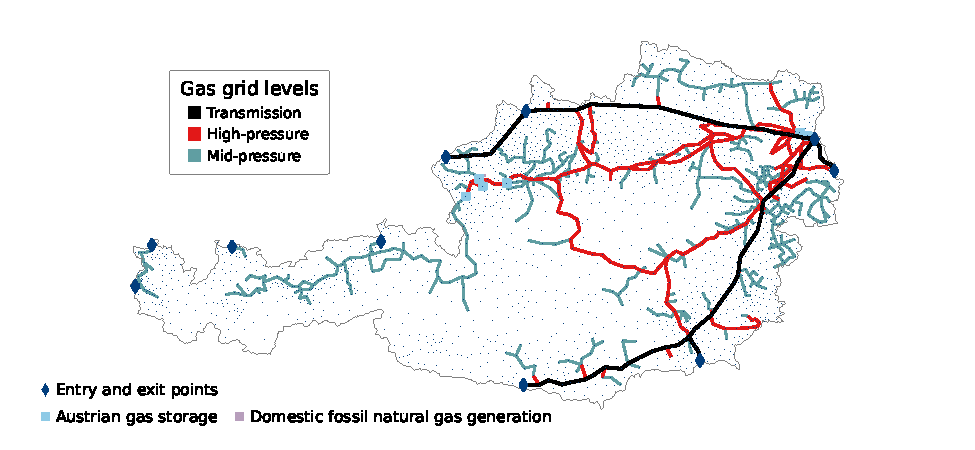
\includegraphics[width=1\linewidth]{figures/method/existing_gas_grid/2023_existing_natural_gas_grid.pdf}
	\caption{Representation of the existing natural gas grid in Austria in the model. \added{Based on information from} \cite{econtrol_grid1,aggm_agid}.}
	\label{method:existing_gas_grid}
\end{figure}

Entry and exit points connecting the Austrian gas grid with the neighboring gas grids, the Austrian gas storage capacities and the domestic fossil natural gas generation are taken into account, in addition to the existing natural gas grid being represented in the model by 738 pipeline sections (lines) and 657 supply and demand points (nodes).\vspace{0.3cm}

In total, the existing natural gas grid, serving as the starting gas grid, consits of transmission, high-pressure, and mid-pressure pipelines that have in total a length of around \SI{6700}{km}. Below is a brief description of how the authors of the study determined the existing Austrian gas grid in their model as a third party. The fact is that data about gas grids, especially at the distribution grid level, is scarcely accessible to the public. However, data is available for the transmission grid level and for gas storage, for example, published by ENTSO-G \cite{entsog}. At the distribution grid levels, data was partly provided in the form of shapefiles (which is a digital vector storage format for storing geographic location and associated attribute information, such as transport capacities in the context here) upon request (see \cite{zwickl2023design}). Where data on the distribution grid was not available, the location of the high-pressure and mid-pressure pipelines is determined manually (i.e., by comparison with publicly available maps and illustrations from the Austrian energy regulator \cite{econtrol_grid1}) and transport capacities are estimated. This includes the age structure of gas pipelines, for which some information is available on the Internet. The latter can be found, for example, on the websites of the distribution grid operators. The resulting Austrian gas grid, consisting of gas pipelines at the transmission, high-pressure, and mid-pressure grid levels, is then overlaid on the map of Austria at the level of municipalities. There are 2095 Austrian municipalities in total according to the NUTS nomenclature. So those municipalities with natural gas demand and crossing the resulting gas grid are a node in the gas grid graph. As mentioned, there are 657 of such nodes building the existing Austrian gas grid in the model. The connection between two of these nodes are one of the 738 pipeline sections in the model. If a municipality with natural gas demand does not have an intersection with a gas pipeline of the existing grid (e.g., because only a low-pressure pipeline connects is available, which is not considered in the existing gas grid), the demand (and/or generation) is assigned to the nearest node with the shortest distance. 

\subsection{Scenarios}\label{scenarios}
In the absence of a holistic modeling view of the energy system across all energy sectors and sources in this study, the scenarios are of particular importance. In a precise level of energy source use that is modeled in an optimal way in these holistic modeling approaches, the scenarios and their underlying narrative define the degree of electrification, or the use of renewable natural gas and hydrogen in the process of decarbonizing the energy system when replacing fossil natural gas. Based on the degree of electrification, natural gas and hydrogen, this study here does not guarantee, as it is also not the focus, optimality regarding the use of the different energy carriers in a decarbonized Austrian energy system, with the scenarios providing estimates particularly for the development of the amounts of natural gas demand and generation (incl. import and export from and to neighboring countries). The scope is much more on: if we have these amounts and localization of natural gas demand and generation in Austria given, which gas grid is required for balancing both.\vspace{0.3cm}

With this in mind, four different scenarios are defined. They are called "Electrification", "Green Gas", "Decentralized Green Gas" and "Green Methane" and span a wide range of the development of gas demand and generation in Austria. All the four scenarios are based on published national decarbonization scenarios for the Austrian energy system. For example, the scenario Electrification is based on the 2023 \textit{Transition Szenario}, recently fundamentally updated and published by the \textit{Environment Agency Austria} \cite{umweltbundesamt}. Figure \ref{fig:scenario_narratives} gives a characterization of the four scenarios by in total eight dimensions, allowing a qualitiative comparison regarding natural gas demand, generation and its spatial concentration. Based on this qualitative overview of the four scenarios, the natural gas demand is the lowest in the scenario Electrification (Elec) with \SI{7.2}{TWh}, and the highest natural gas demand is in the scenario Green Methane (GM) with \SI{84.2}{TWh}, where we see in Table \ref{tab:scenario_demand} and \ref{tab:scenario_generation} the quantitative numbers of natural gas demand and domestic generation in the four scenarios in 2040, respectively. Latter, for instance, accounts for \SI{91.9}{\%} of the natural gas demand in Austria 2022. 

\definecolor{Gray}{gray}{0.95}
\begin{table}[h]
	\centering
	\setlength{\extrarowheight}{1em}
	\resizebox{1\textwidth}{!}{
		\begin{tabular}{lrrrr}
			\toprule
			Scenario & Elec & GG & DGG & GM\\\hline
			Natural gas demand in 2030&\SI{49.8}{TWh}&\SI{60.3}{TWh}&\SI{63.4}{TWh}&\SI{79.4}{TWh}\\
			\textcolor{white}{Natural gas demand} in 2040&\cellcolor{Gray}\SI{7.2}{TWh}&\cellcolor{Gray}\SI{9.5}{TWh}&\cellcolor{Gray}\SI{20.3}{TWh}&\cellcolor{Gray}\SI{84.2}{TWh}\\\hline
			2040's share of 2022's demand&\SI{9.0}{\%}&\SI{11.0}{\%}&\SI{23.5}{\%}&\SI{91.9}{\%}\\\hline
			Reference for the demand&\cite{umweltbundesamt}&\cite{Energieagentur}&\cite{Energieagentur}&\cite{Energieagentur}\\
			\bottomrule
	\end{tabular}}
	\caption{Natural gas demand in Austria the four scenarios in 2030 and 2040 and comparison with the demand in 2022. Values taken and build on decarbonization scenarios developed and published by the \textit{Environment Agency Austria} \cite{umweltbundesamt} and \textit{Austrian Energy Agency} \cite{Energieagentur}. Abbreviations: Electrification (Elec), Green Gases (GG), Decentralized Green Gases (DGG), Green Methane (GM).}
	\label{tab:scenario_demand}
\end{table}

For the interpretation of the study results, three aspects in the scenario definition are crucial. Therefore, they are highlighted here in particular: 

\begin{itemize}
	\item By the target year 2040, only renewable gases are used to supply Austria's natural gas demand in all the four scenarios. This applies to both the domestic generation (i.e., biomethane based on biogas and synthetic natural gas based on renewable energy) and to the imports of natural gas.
	\item In three of the four scenarios (Electrification, Green and Decentralized Green Gases), the renewable domestic natural gas generation supplies the complete demand. As a consequence, there is a national balance between generation and demand in Austria 2040 and no imports are needed. 
	\item In these three chosen scenarios, the transmission grid only transports gas across Austria and is not used to meet demand in Austria, as, where no imports are needed, the transmission and distribution grids are physically and economically separate. The separation of the two grids is reflected in the results in that the costs of the transmission grid are borne by Austrian consumers only when imports are needed. This is only the case in the GM scenario.\footnote{Whether or not the physical separation of the transmission and distribution grids in such case where there is no need for imports is reasonable for energy security reasons is beyond the scope of this paper.}
\end{itemize}

\begin{table}[h]
	\centering
	\setlength{\extrarowheight}{1em}
	\resizebox{1\textwidth}{!}{
		\begin{tabular}{lrrrr}
			\toprule
			Scenario & Elec & GG & DGG & GM\\\hline
			Natural gas generation in 2030&\SI{4.0}{TWh}&\SI{5.0}{TWh}&\SI{5.0}{TWh}&\SI{5.0}{TWh}\\
			\cellcolor{white}\textcolor{white}{Natural gas generation} in 2040&\cellcolor{Gray}\SI{7.2}{TWh}&\cellcolor{Gray}\SI{9.5}{TWh}&\cellcolor{Gray}\SI{20.3}{TWh}&\cellcolor{Gray}\SI{30.2}{TWh}\\\hline
			2040's share of biomethane&\SI{7.2}{TWh}&\SI{9.5}{TWh}&\SI{9.5}{TWh}&\SI{9.5}{TWh}\\
			2040's share of synthetic gas&\SI{0}{TWh}&\SI{0}{TWh}&\SI{10.7}{TWh}&\SI{20.6}{TWh}\\
			2040's share of fossil gas&\SI{0}{TWh}&\SI{0}{TWh}&\SI{0}{TWh}&\SI{0}{TWh}\\\hline
			2040's share of the demand&\SI{100}{\%}&\SI{100}{\%}&\SI{100}{\%}&\SI{35.9}{\%}\\\hline
			Reference for the generation&\cite{umweltbundesamt}&\cite{Energieagentur}&\cite{Energieagentur}&\cite{Energieagentur}\\
			\bottomrule
	\end{tabular}}
	\caption{Domestic renewable natural gas generation in Austria 2030 and 2040. Three of the four scenarios consider a complete supply of the national natural gas demand by renewable domestic generation. Values taken and build on decarbonization scenarios developed and published by the \textit{Environment Agency Austria} \cite{umweltbundesamt} and \textit{Austrian Energy Agency} \cite{Energieagentur}. Abbreviations: Electrification (Elec), Green Gases (GG), Decentralized Green Gases (DGG), Green Methane (GM).}
	\label{tab:scenario_generation}
\end{table}

Finally, three aspects should be pointed out. Visualizations of the domestic gas generation and demand are given in \ref{app:visualization}. Those maps combined with the qualitative overview of the scenarios given in Figure \ref{fig:scenario_narratives} should sufficiently explain the scenarios for this paper's aim. Whereas the transit of natural gas through Austria is taken from existing modeling studies \cite{frontier2020, frontier2023}, regarding the transit of natural gas, except for the scenario Green Methane (GM), it is assumed that the domestic generation covers the national demand in 2040. In addition, the repurposing of existing gas pipelines for hydrogen transport is also taken from existing studies published by the Austrian gas grid operator \cite{aggm_agid}. 

\afterpage{\clearpage}
\begin{sidewaysfigure}[h]
	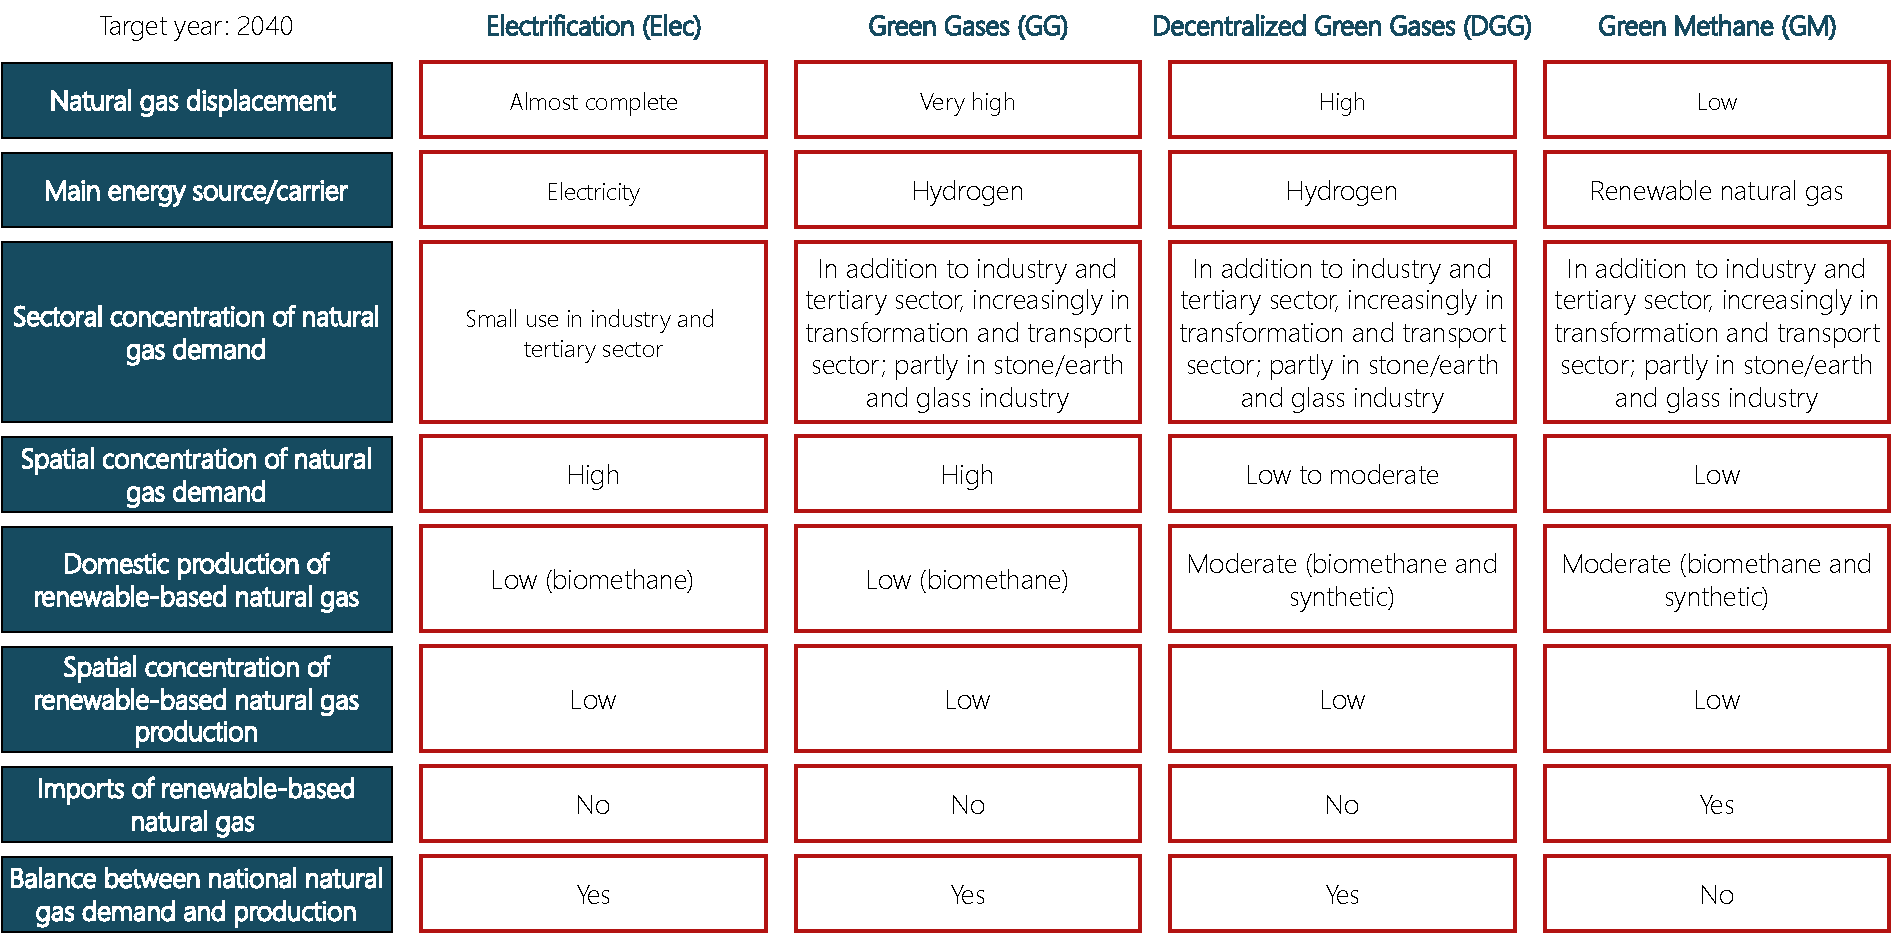
\includegraphics[width=1\linewidth]{figures/method/scenario_narrative.pdf}
	\caption{Overview of the most relevant dimensions characterizing the four scenarios. Storylines and narratives of the scenarios build on decarbonization scenarios developed and published by the \textit{Environment Agency Austria} \cite{umweltbundesamt} and \textit{Austrian Energy Agency} \cite{Energieagentur}.}
	\label{fig:scenario_narratives}
\end{sidewaysfigure} 

\newpage
\section{Results}\label{results}
This section shows the main findings of the Austrian case study. As described above, results for the four scenarios Electrification (Elec), Green Gases (GG), Decentralized Green Gases and Green Methane (GM) are presented. It is structured in three parts. First, Sections \ref{res_grid2030} and \ref{res_grid2040} present the Austrian gas grid in 2030 and 2040, respectively. Section \ref{res_grid_charges} focuses on the grid costs and elaborates on the grid charges for end customers in 2040, with the quantitative results for grid length, operating, and investment costs being presented for both target years in detail.

\subsection{Austrian gas grid in 2030}\label{res_grid2030}
The Austrian gas grid in 2030 is shown in Figure \ref{fig_grid_2030}. It is the same in all four scenarios and is very similar to the initial grid in 2025, only slightly smaller. 

\begin{figure}[h]
	\centering
	\includegraphics[width=1\linewidth]{figures/results/gas_grid_2030_all_scenarios_cleaned.pdf}
	\caption{Austrian gas grid in 2030 at the transmission (blue), high-pressure (red) and mid-pressure (green) pressure levels in all four scenarios.}
	\label{fig_grid_2030}
\end{figure}

The main reason for the slight reduction of the grid length is the use of redundancies and duplicate structures in the grid as a result of declining gas demand. Table \ref{tab_compare_initial_2030} shows the reduction in the grid length at the high-pressure and mid-pressure levels in the four scenarios. 

\begin{table}[h]
	\centering
	\setlength{\extrarowheight}{.5em}
	\resizebox{0.9\textwidth}{!}{
		\begin{tabular}{lccccc}
			\toprule
			& 2025 & \multicolumn{4}{c}{2030}\\\cmidrule(lr){2-2}\cmidrule(lr){3-6}
			Pressure level & Initial grid & Elec & GG & DGG & GM\\\cmidrule(lr){1-2}\cmidrule(lr){3-6}
			\multirow{2}{*}{High-pressure} & \multirow{2}{*}{\SI{1449}{km}} & \SI{-172}{km}  & \SI{-142}{km} & \SI{-142}{km}  & \SI{-131}{km}\\
			&  & (\SI{-11.9}{\%}) & (\SI{-9.8}{\%}) & (\SI{-9.8}{\%}) & (\SI{-9.0}{\%})\\\hdashline
			\multirow{2}{*}{Mid-pressure} & \multirow{2}{*}{\SI{3218}{km}} & \SI{-283}{km}  & \SI{-200}{km} & \SI{-186}{km}  & \SI{-208}{km}\\
			& & (\SI{-8.8}{\%}) & (\SI{-6.2}{\%}) & (\SI{-5.8}{\%}) & (\SI{-6.5}{\%})\\
			\bottomrule
	\end{tabular}}
	\caption{Absolute and relative reduction in the length of the gas grid at the high-pressure and mid-pressure levels by 2030 compared to the initial grid in 2025. Abbreviations: Electrification (Elec), Green Gases (GG), Decentralized Green Gases (DGG), Green Methane (GM).}
	\label{tab_compare_initial_2030}
\end{table}

The reduction in the grid length at the high-pressure level varies between \SI{-131}{km} and \SI{-172}{km} in the GM and Elec scenarios respectively. The reduction in the grid length at the mid-pressure level varies between \SI{-186}{km} and \SI{-283}{km} in the DGG and Elec scenarios, respectively. Removing redundant gas pipelines reduces the operating costs of the grid.\footnote{In reality, these gas pipelines, especially at the transmission and high-pressure levels, can form the core of a hydrogen grid. For further details, see for example, the plans for the Austrian hydrogen grid by 2030 published by the Austrian gas grid operator \cite{aggm_agid}.} The operating costs of the gas grid, which are mainly fixed pipeline costs, decrease compared to the initial grid in 2025 and are around \SI{110}{MEUR} in all four scenarios in 2030. By 2030, virtually no gas pipelines are decommissioned due to aging or because the pipeline is no longer used to transport gas, while it is important to note that energy costs for the compressor are not included in all four scenarios. In total, those investments vary by 2030 between \SI{15}{MEUR} and \SI{18}{MEUR} in the Elec and GM scenarios, respectively, with its being of note that the rather young Austrian grid age also leads to very low replacement investments into the gas grid. Note that in the model presented in this paper, replacement investment is necessary when a pipeline reaches its technical lifetime of \SI{75}{years}. At this point, the model decides whether to invest in replacing the pipeline or to decommission it age-related. 

\subsection{Austrian gas grid in 2040}\label{res_grid2040}
The Austrian gas grid in 2040 differs significantly between the four scenarios, within which four different gas grids emerge. These four grids are mainly determined by the assumptions of the underlying scenarios. Figures \ref{fig_grid_2040_small} (Elec scenario) and \ref{fig_grid_2040_large} (GM scenario) show the smallest and largest gas grids in terms of grid length. 

\begin{figure}[h]
	\centering
	\includegraphics[width=1\linewidth]{figures/results/gas_grid_2040_elec.pdf}
	\caption{Austria's smallest gas grid by 2040 in the scenario Electrification (Elec). Colors: transmission (blue), high-pressure (red) and mid-pressure (green).}
	\label{fig_grid_2040_small}
\end{figure}

The smallest grid is in the Elec scenario and the largest in the GM scenario. They lie between the two extreme grids in terms of size. Table \ref{tab_compare_initial_2040} quantifies the size of the gas grids in 2040 in all the four scenarios by comparing the absolute length of the grids, where in absolute numbers, the reduction of grid length at the mid-pressure level is more significant than at the high-pressure level, as well as the absolute and relative reduction of grid lengths compared to the initial grid in 2025. In particular, the reduction in the grid length at the mid-pressure level is equally greatest in the two scenarios Elec and GG with \SI{-1316}{km} (\SI{-40.9}{\%} compared to the initial grid in 2025). The smallest reduction in length at the mid-pressure level among the four scenarios is with \SI{-811}{km} (\SI{-25.2}{\%} compared to the initial grid in 2025) in the DGG scenario. 

\begin{figure}[h]
	\centering
	\includegraphics[width=1\linewidth]{figures/results/gas_grid_2040_gm.pdf}
	\caption{Austria's largest gas grid by 2040 in the scenario Green Methane (GM). Colors: transmission (blue), high-pressure (red) and mid-pressure (green).}
	\label{fig_grid_2040_large}
\end{figure}

The main reason here for the relatively small reduction in the mid-pressure grid length is the significant decentralized generation and injection of domestic renewable gas. 

\begin{table}[h!]
	\centering
	\setlength{\extrarowheight}{.5em}
	\resizebox{1\textwidth}{!}{
		\begin{tabular}{llrrrr}
			\toprule
			& & \multicolumn{4}{c}{2040}\\\cmidrule(lr){3-6}
			Pressure level & Indicator & \multicolumn{1}{c}{Elec} & \multicolumn{1}{c}{GG} & \multicolumn{1}{c}{DGG} & \multicolumn{1}{c}{GM}\\\cmidrule(lr){1-2}\cmidrule(lr){3-6}
			\multirow{3}{*}{High-pressure} & Abs. grid length in 2040& \SI{964}{km}  & \SI{965}{km} & \SI{974}{km}  & \SI{1105}{km}\\
			 & Abs. reduction to 2025 & \SI{-485}{km}  & \SI{-484}{km} & \SI{-475}{km}  & \SI{-344}{km}\\
			 & Rel. reduction to 2025 & \SI{-33.5}{\%}& \SI{-33.4}{\%}& \SI{-32.8}{\%}&\SI{-23.7}{\%}\\\hdashline
 			\multirow{3}{*}{Mid-pressure} & Abs. grid length in 2040& \SI{1902}{km}  & \SI{1902}{km} & \SI{2407}{km}  & \SI{2331}{km}\\
			 & Abs. reduction to 2025 & \SI{-1316}{km}  & \SI{-1316}{km} & \SI{-811}{km}  & \SI{-887}{km}\\
			 & Rel. reduction to 2025 & \SI{-40.9}{\%}& \SI{-40.9}{\%}& \SI{-25.2}{\%}&\SI{-27.6}{\%}\\
			\bottomrule
	\end{tabular}}
	\caption{Absolute length of the grids 2040 in the four scenarios as well as the absolute and relative reduction of grid lengths compared to the initial grid in 2025 at the high-pressure and mid-pressure levels. Abbreviations: Electrification (Elec), Green Gases (GG), Decentralized Green Gases (DGG), Green Methane (GM).}
	\label{tab_compare_initial_2040}
\end{table}

The domestic injection leads to an increased use of mid-pressure pipelines. Figure \ref{fig_reduction_waterfall} shows the grid length in the two extreme scenarios Elec (top) and GM (bottom) at high-pressure (left) and mid-pressure (right) levels. It highlights the reduction in grid length by 2030 and 2040. The grid length in 2025 is shown on the far left and in 2040 on the far right. 

\begin{figure}[h]
	\begin{subfigure}[c]{0.5\textwidth}
		\centering
		\includegraphics[width=1\linewidth]{figures/results/waterfall/waterfall_elec_high.pdf}
		\vspace{-0.6cm}
		\subcaption{Elec | High-pressure}
		\label{Fig:a}
	\end{subfigure}
	\begin{subfigure}[c]{0.5\textwidth}
		\centering
		\includegraphics[width=1\linewidth]{figures/results/waterfall/waterfall_elec_mid.pdf}
		\vspace{-0.6cm}
		\subcaption{Elec  | Mid-pressure}
		\label{Fig:b}
	\end{subfigure}
	\newline
	\newline
	\newline
	\begin{subfigure}[c]{0.5\textwidth}
		\centering
		\includegraphics[width=1\linewidth]{figures/results/waterfall/waterfall_gm_high.pdf}
		\vspace{-0.6cm}
		\subcaption{GM | High-pressure}
		\label{Fig:c}
	\end{subfigure}
	\begin{subfigure}[c]{0.5\textwidth}
		\centering
		\includegraphics[width=1\linewidth]{figures/results/waterfall/waterfall_gm_mid.pdf}
		\vspace{-0.6cm}
		\subcaption{GM | Mid-pressure}
		\label{Fig:d}
	\end{subfigure}
	\caption{Comparison of the Austrian gas grid in 2025 and 2040 in the extreme scenarios Electrification (Elec) and Green Methane (GM) at high-pressure and mid-pressure levels. In the Elec and GM scenarios, the smallest and the largest gas grids are obtained in terms of the size of the grids.}
	\label{fig_reduction_waterfall}
\end{figure}

The operating costs of the gas grid decrease compared to 2025. They vary between \SI{87.5}{MEUR} and \SI{93.0}{MEUR} in the Elec and GM scenarios, respectively. With the remaining costs being accounted by the high-pressure and mid-pressure level, \SI{50.0}{MEUR} (the same in all four scenarios) are accounted for the transmission level. Figure \ref{fig_grid_repl_inv} shows the total replacement investments in the gas grid in the four scenarios. It includes the replacement investments in 2030 mentioned in Section \ref{res_grid2030} above. The lowest total replacement investments are in the scenarios GG and Elec with \SI{143.0}{MEUR} and \SI{146.0}{MEUR} respectively. The highest replacement investments are in the GM scenario with \SI{185.0}{MEUR}. 

\begin{figure}[h]
	\centering
	\includegraphics[width=0.8\linewidth]{figures/results/total_replacement_inv/replace_inv_2040.pdf}
	\caption{Total replacement investments in the Austrian gas grid until 2040 in the four scenarios.}
	\label{fig_grid_repl_inv}
\end{figure}

The off-grid solution is not used in the four scenarios, with the model not choosing the off-grid solution due to its high costs, except in very few cases, with this also being true when meager amounts of gas are transported through gas pipelines. The economic trade-off between a scarcely utilized gas pipeline and the off-grid solution is illustrated in Figure \ref{line_and_point} in \ref{app_off_grid}.

\subsection{Grid charges for customers in 2040}\label{res_grid_charges}
This section presents an analysis of the cost-effectiveness of the gas grid in four different scenarios. In average grid costs serving as a basis for estimating grid charges for customers in 2040, the average grid costs are calculated by dividing the total annual grid costs by the gas demand supplied. It should be noted that determining grid charges based on minimizing system costs must be viewed with caution, although regulatory mechanisms often rely on approaches that aim to minimize system costs, as a grid charge regulation process must also take other considerations into account. Therefore, it is important to consider and interpret the following results from this perspective. In particular, the different grid costs provide a different perspective on comparing the four scenarios.\vspace{0.3cm}

Noting that the horizontal axis is the renewable gas demand supplied by the grid in TWh, Figure \ref{fig_grid_charges} shows the (average) grid costs in 2040 in the four different scenarios. The Elec scenario, as it has the lowest gas demand of the four scenarios, is therefore on the far left. At the same time, the GM scenario, which has the highest gas demand among the scenarios, is on the far right. 

\begin{figure}[h]
	\centering
	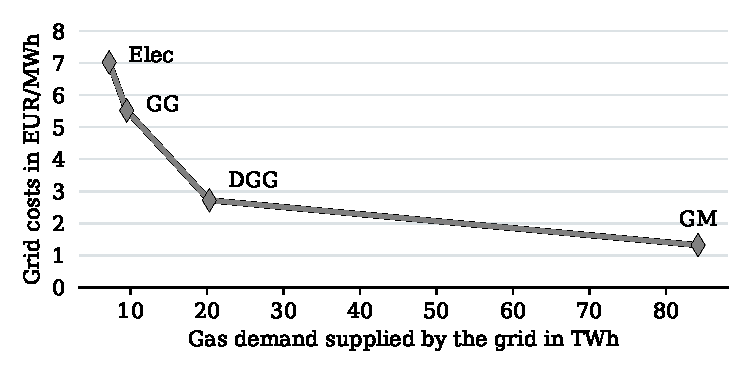
\includegraphics[width=1\linewidth]{figures/results/grid_charges/grid_charges.pdf}
	\caption{Grid costs in the four scenarios Electrification (Elec), Green Gases (GG), Decentralized Green Gases (DGG) and Green Methane (GM).}
	\label{fig_grid_charges}
\end{figure}

It is shown that the grid costs are the highest in the Elec scenario with \SI{7.0}{EUR \per MWh} and the lowest in the GM scenario with \SI{1.3}{EUR \per MWh}. The grid costs and its components of operating costs at the different pressure levels and gas demand supplied are summarized in Table \ref{tab_components_grid_costs}. Note that the transmission operating costs accounted for customers in these scenarios are zero, as the three scenarios Elec, GG and DGG assume a separation between the transmission and distribution grids (i.e., high and medium pressure levels). Consequently, it is assumed that customers requesting gas transport through Austria at the transmission level bear these costs. A comparison of the average grid costs with the current grid charges in Austria shows that these are increasing significantly in three of the four scenarios. The current grid charges at the mid-pressure level in Austria are around \SI{1.7}{EUR \per MWh} \cite{econtrol_gas_charges}.

\begin{table}[h!]
	\centering
	\setlength{\extrarowheight}{.5em}
	\resizebox{0.85\textwidth}{!}{
		\begin{tabular}{lrrrr}
			\toprule
			& \multicolumn{4}{c}{2040}\\\cmidrule(lr){2-5}
			Components for calculating grid costs & Elec & GG & DGG & GM\\\hline
			Transmission operating costs in MEUR & 0 & 0 &0  & \SI{50}{}\\
			Distribution operating costs in MEUR & \SI{37.5}{} & \SI{39.3}{} & \SI{40.2}{} & \SI{43.0}{}\\
			Capital costs per year in MEUR & \SI{13.0}{} & \SI{13.1}{} & \SI{15.0}{} & \SI{18.3}{}\\
			Gas demand supplied in TWh & \SI{7.2}{} & \SI{9.5}{} & \SI{20.3}{} & \SI{84.2}{}\\\hline
			Grid costs in EUR/MWh & \SI{7.0}{} & \SI{5.5}{} & \SI{2.7}{} & \SI{1.3}{}\\
			\bottomrule
	\end{tabular}}
	\caption{Average grid costs and their components of operating costs and capital costs. The distribution operating costs encompass the high-pressure and mid-pressure levels. Separation between the transmission and distribution grids result in accounting no transmission operating costs for the customers.}
	\label{tab_components_grid_costs}
\end{table}

 Only in the GM scenario, where the supply depends on massive renewable imports, do the grid costs remain around or slightly below this value. In the results of the other three scenarios, the increase in grid costs is driven by the high operating costs of the distribution grid with comparatively low demand volumes and capital costs. Necessary due to the aging of the (otherwise already fully depreciated) existing grid, the (annual) capital costs in 2040 result essentially from the replacement investments made by then. As mentioned, a technical lifetime of the pipelines of \SI{75}{years} is assumed. A possible window for reducing grid costs opens, as a more extended operation of pipelines (e.g., technical lifetime between 90 and \SI{100}{years}) could reduce the share of capital costs in the grid costs; in extreme cases even go toward zero. Such a measure of a longer operating life of pipelines is certainly considered in practice, especially against the background of declining transport volumes. This is because transport volumes determine the operating pressure levels, which determine the pipelines' wear and tear. While replacement investments due to aging could be saved, lowering the operating pressure levels compared to today's could extend the technical lifetime\footnote{In addition, lowering the operating pressure levels also affects and supports domestic renewable gas generation. On the one hand, generation plants require less energy to compress their gas, and on the other hand, their connection costs are reduced, as the costs are highly dependent on the pressure levels in the grid. For more information from the field, see \cite{biogas_einspeisung}.}. Figure \ref{fig_grid_charges_no_capex} shows the impact on the grid costs if an extension of the pipelines' technical lifetime to \SI{90}{}-\SI{100}{years} is taken into account. With grid costs consequently going down in all the four scenarios, the lifetime extension leads to no replacement investments and the current pipelines can remain in operation. The highest reduction in grid costs is with \SI{-1.8}{EUR/MWh} in the Elec scenario. The latter is the one with initially the highest grid costs. The smallest reduction in grid costs is with \SI{-0.2}{EUR/MWh} in the GM scenario.

\begin{figure}[h]
	\centering
	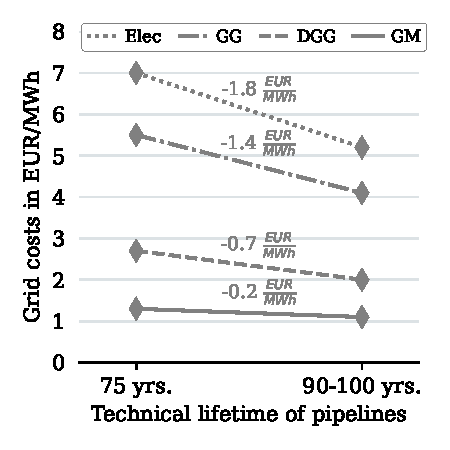
\includegraphics[width=0.6\linewidth]{figures/results/grid_charges_development/cleaned_grid_charges.pdf}
	\caption{Comparison of grid costs in 2040 for a technical lifetime of pipelines of \SI{75}{years} (left) and 90-\SI{100}{years} (right).}
	\label{fig_grid_charges_no_capex}
\end{figure}

\section{Synthesis}\label{synthesis}
With respect to the three research questions posed in this paper, the generated results show some expected and some unexpected results. As expected, by also looking at the future demand volumes of natural and renewable gas, the Austrian gas grid in a decarbonized energy system will shrink. However, the extent of shrinking, varies though between the decarbonization scenarios, but is generally significantly lower than expected when looking solely at the future demand volumes. Main driver is the integration of decentralized renewable gas generation (biomethane and synthetic gas) and the fact that stand-alone supply options (trucking and on-site gas storage) are not competitive with piped supply. Nevertheless, in terms of grid costs, it is primarily the fixed costs of the existing gas grid (rather than the capital costs of the refurbished gas pipelines) that lead to a, in some scenarios, significant increase in average grid costs compared to the status quo (e.g., fivefold increase in the scenario with a high electrification of the energy system). Only in the scenario with continued high use of natural gas (trough imports of decarbonized natural gas) do average gas grid costs remain similar to those of today's gas grids.\vspace{0.3cm}

Assuming ambitious national climate targets (e.g. decarbonization of the gas sector), the findings discussed above and the results obtained in general can be generalized in the sense that they are valid for those countries with a similarly high expectation for renewable gas generation. In Europe, for instance, it is likely that the results for countries such as Germany, Italy and France might look similar. These generalizations are, of course, more to be understood as qualitative statements and would require detailed analyses in any case. The specific geographical location of the renewable gas (and demand) in the analysis have proven to be too determining and crucial.\vspace{0.3cm}

With regard to the limitations of the study, two aspects should be mentioned and taken into account when interpreting the results. First, the results are largely scenario driven. For example, natural gas demand and renewable gas generation are determined by the scenarios and then used exogenously in the gas network modeling. In essence, the demand and generation volumes are inelastic to gas network costs. Second, based on the gas network costs, an indication of the end customer costs is given. In this context, the treatment of (average) gas network and retail costs is relatively simplistic and could mislead the inattentive reader. Again, the average network costs are used to give a quantitative indication of how network costs for retail customers may develop in the future. As always with this type of analysis, especially when dealing with sensitive data of the existing energy system, such as gas network information, the number of assumptions that have to be made due to lack of information by the researcher and third parties should be taken into account when interpreting the present results. 
% Regarding the limitations of the study, among others, two aspects should be mentioned and taken into account when interpreting the results obtained. Firstly, the results are to a large extent scenario driven. For example, natural gas demand and renewable gas generation are determined by the scenarios and then used in the gas grid modeling exogenously. Essentially, the demand and generation volumes are inelastic to the gas grid costs. Secondly, based on the gas grid costs, an indication is given for end customers' costs. In this context, the way (average) gas grid and end customers' costs are treated is comparatively simplistic and could mislead the inattentive reader. Again, the average grid costs are used to give an quantitative indication of how the grid costs for end customers may develop in the future. As always in these kind of analyses, in particular when it comes to sensitive data of the existing energy system, such as gas grid information, the bunch of assumptions that have to be made because of a lack of information as a researcher and third-party should be taken into account when interpreting the present results. 






























\section{Conclusions}\label{conclusions}
In many countries, the debate about using natural gas grids in sustainable energy systems has erupted, with the future of natural gas grids being one of the most pressing issues in realizing energy system decarbonization, at least in Europe. This paper contributes to the discussion by conducting a detailed national case study. While in particular, the case study is used to provide detailed insights into a well-developed gas grid with an expected significant decrease in natural gas demand and a significant increase in decentralized renewable gas generation, at the same time a techno-economic analysis of the Austrian gas grid to 2040 in four decarbonization scenarios is carried out.\vspace{0.3cm}

Austria's natural gas grids will shrink in the future; the natural gas demand will likely be spatially concentrated and restricted to large consumers, such as industrial facilities, and the level of shrinkage depends primarily on the level of integration of renewable gas and not on the level of demand for natural gas. The size of gas grids will be determined, on the one hand, by the quantities of domestic generation (and demand), on the other hand, by their spatial location. If an area-wide integration of domestic renewable gases into the gas grid happens, a significant increase in average grid costs and grid tariffs for the end customers must be expected. The aging of the existing gas grid and related refurbishment investments play a relatively minor role in the gas grid costs, as fixed costs mainly determine them. At the same time, off-grid solutions such as trucking and on-site storage are not competitive with the gas grid (even if the gas grid is very low utilized).\vspace{0.3cm}

The final finding on the increase in gas grid costs for large-scale renewable gas injection can be a starting point for further work. The questions that arise are not only who bears the high gas grid costs in such a case and what influence they have on the end customer's decision whether or not it is economical to stick with natural gas as an energy source, but also how synergies between renewable gas generators and natural gas demand can be exploited. The latter means exploring the spatial interplay of local generation and demand, for example, by forming regional renewable gas clusters. \added{One of the following questions is certainly how energy policy instruments can support these regional renewable gas clusters in an economically efficient way. At the same time, security of supply concerns need to be addressed in cases where these clusters are operated similarly to an islanded grid without significant supply redundancy (e.g., a regional renewable gas cluster in island mode with only one generation site could represent an extreme implementation).} Additionally, future research should examine the need for a dedicated hydrogen grid. That is a necessary complement to the present study, as hydrogen blending is not considered, and thus, hydrogen transport takes place in a separate grid if needed.\vspace{0.3cm}
















\section*{Declaration of interests}
None.
\section*{Data availability}
The original data used in this study are publicly available. The compiled dataset is published on Zenodo at \textcolor{gray}{(Link as soon as the paper has been published).} 
\section*{Code availability}
The code is published under an open license on GitHub at \textcolor{gray}{(Link as soon as the paper has been published).}

\section*{Acknowledgments}
This work was supported by the Federal Ministry Republic of Republic Austria
for Climate Action, Environment, Energy, Mobility, Innovation and Technology under the project Gas-Infra-AT-2040 ("The future role of gas infrastructure in a climate-neutral Austria by 2040"). The authors acknowledge TU Wien Bibliothek for financial support through its Open Access Funding Programme.


\bibliography{mybibfile}
\appendix
\setcounter{table}{0}
\setcounter{figure}{0}
\newpage
\section{Gas grid parameters and empirical scaling}\label{paramter}
The economic parameters and assumptions for the gas grid (and its pipelines) and the alternative off-grid solution (trucking and on-site gas storage) are summarized in Table \ref{tab:parameters} and Table \ref{tab:off_grid} respectively. 

\begin{table}[h]
	\centering
	\setlength{\extrarowheight}{1em}
	\resizebox{1\textwidth}{!}{
			\begin{tabular}{p{0.2\linewidth}|p{0.225\linewidth}|p{0.25\linewidth}|p{0.325\linewidth}}
				\toprule
				\raggedright Investment costs & \raggedright Pipeline (Transmission) & \raggedright \SI{120}{EUR \per MW \per km} and \SI{2200}{EUR \per m} & \raggedright DN1000; average operating pressure approx. \SI{55}{bar}; Gas flow velocity approx. \SI{10}{m \per s}\arraybackslash\\\hline
				\raggedright Investment costs & \raggedright Pipeline (High-Pressure) & \raggedright \SI{170}{EUR \per MW \per km} and \SI{1590}{EUR \per m} & \raggedright DN800; average operating pressure approx. \SI{55}{bar}; Gas flow velocity approx. \SI{9}{m \per s}; Length \SI{150}{km}\arraybackslash\\\hline
				\raggedright Investment costs & \raggedright Pipeline (Mid-Pressure) & \raggedright \SI{2135}{EUR \per MW \per km} and \SI{850}{EUR \per m} & \raggedright DN300; average operating pressure approx. \SI{23}{bar}; Gas flow velocity approx. \SI{12}{m \per s}; Length \SI{25}{km}\arraybackslash\\\hline
				\raggedright Fixed costs (excl. gas compressor energy)& \raggedright Pipeline (Transmission) & \raggedright \SI{430}{EUR \per MW} & \raggedright \SI{1.8}{\%} of the investment costs of a transmission pipeline (typical length of \SI{200}{km})\arraybackslash\\\hline
				\raggedright Fixed costs & \raggedright Pipeline (High-Pressure) & \raggedright \SI{460}{EUR \per MW} & \raggedright \SI{1.8}{\%} of the investment costs of a transmission pipeline (typical length of \SI{150}{km})\arraybackslash\\\hline
				\raggedright Fixed costs & \raggedright Pipeline (Mid-Pressure) & \raggedright \SI{960}{EUR \per MW} & \raggedright \SI{1.8}{\%} of the investment costs of a transmission pipeline (typical length of \SI{25}{km})\arraybackslash\\\hline
				\raggedright WACC & \raggedright Pipelines (all grid levels) & \raggedright \SI{5}{\%} & \raggedright Weighted average cost of capital (WACC)\arraybackslash\\\hline
				\raggedright Amortization period & \raggedright Existing pipelines (all grid levels) & \raggedright \SI{30}{years} & \raggedright Linear depreciation\arraybackslash\\\hline
				\raggedright Amortization period & \raggedright Refurbished pipelines (all grid levels) & \raggedright \SI{20}{years} & \raggedright Linear depreciation\arraybackslash\\\hline
				\raggedright Technical lifetime & \raggedright Existing pipelines (all grid levels) & \raggedright \SI{70}{years} & \arraybackslash\\\hline
	\end{tabular}}
	\caption{Economic parameters for the gas grid}
	\label{tab:parameters}
\end{table}

\begin{table}[h]
	\centering
	\setlength{\extrarowheight}{1em}
	\resizebox{1\textwidth}{!}{
		\begin{tabular}{p{0.2\linewidth}|p{0.225\linewidth}|p{0.25\linewidth}|p{0.325\linewidth}}
			\toprule
			\raggedright Marginal operating costs (demand-side)& \raggedright Off-grid solution (High-Pressure) & \raggedright \SI{390}{EUR \per MWh} & \raggedright Of which \SI{20}{EUR \per MWh} transport costs and \SI{370}{EUR \per MWh} storage costs (two-month gas storage)\arraybackslash\\\hline
			\raggedright Marginal operating costs (demand-side)& \raggedright Off-grid solution (Mid-Pressure) & \raggedright \SI{216.5}{EUR \per MWh} & \raggedright Of which \SI{16.5}{EUR \per MWh} transport costs and \SI{200}{EUR \per MWh} storage costs (one-month gas storage)\arraybackslash\\\hline
	\end{tabular}}
	\caption{Economic parameters for the alternative off-grid solution (trucking and on-site gas storage)}
	\label{tab:off_grid}
\end{table}

\section{Details on today's Austrian natural gas grid}\label{Natural_gas_supply_in_Austria}
A brief overview of today's Austrian gas grid is provided in the following list of bullet points. The following sources are used: \cite{econtrol_grid1, energie}.

\begin{itemize}
	\item Developed over time (first gas pipeline linking Austria, Slovakia, and Italy in 1968);
	\item Important role as a hub for transiting gas through Europe (mainly to Southern and Western Europe, but recently also vice-versa);
	\item Total length of the Austrian transmission grid and distribution grid is around \SI{2000}{km} and \SI{44000}{km} respectively;
	\item Total natural gas demand in Austria per year is around \SI{90}{TWh} (\SI{86.4}{TWh} in 2022 and \SI{94.8}{TWh} in 2021);
	\item Historically, most of Austria's gas demand has been supplied by Russia (average share of \SI{80}{\%} over the last decades).
\end{itemize}

\section{Spatial location of the domestic renewable gas generation and demand 2040}\label{app:visualization}
Figure \ref{generation} and \ref{demand} show the spatial location of the domestic renewable gas generation and natural gas demand in 2030, 2035, and 2040, respectively. 

\begin{figure}[h]
	\centering
	\includegraphics[width=1\linewidth]{figures/appendix/generation.eps}
	\caption{Spatial location of the domestic renewable gas generation in Austria 2030, 2035, and 2040. Abbreviations: Electrification (Elec), Green Gases (GG), Decentralized Green Gases (DGG), Green Methane (GM).}
	\label{generation}
\end{figure}

\begin{figure}[h]
	\centering
	\includegraphics[width=1\linewidth]{figures/appendix/demand.eps}
	\caption{Spatial location of the natural gas demand in Austria 2030, 2035, and 2040. Abbreviations: Electrification (Elec), Green Gases (GG), Decentralized Green Gases (DGG), Green Methane (GM).}
	\label{demand}
\end{figure}

\section{Demonstration of the economic trade-off between piped gas supply and the off-grid solution}\label{app_off_grid}

\begin{figure}[h]
	\centering
	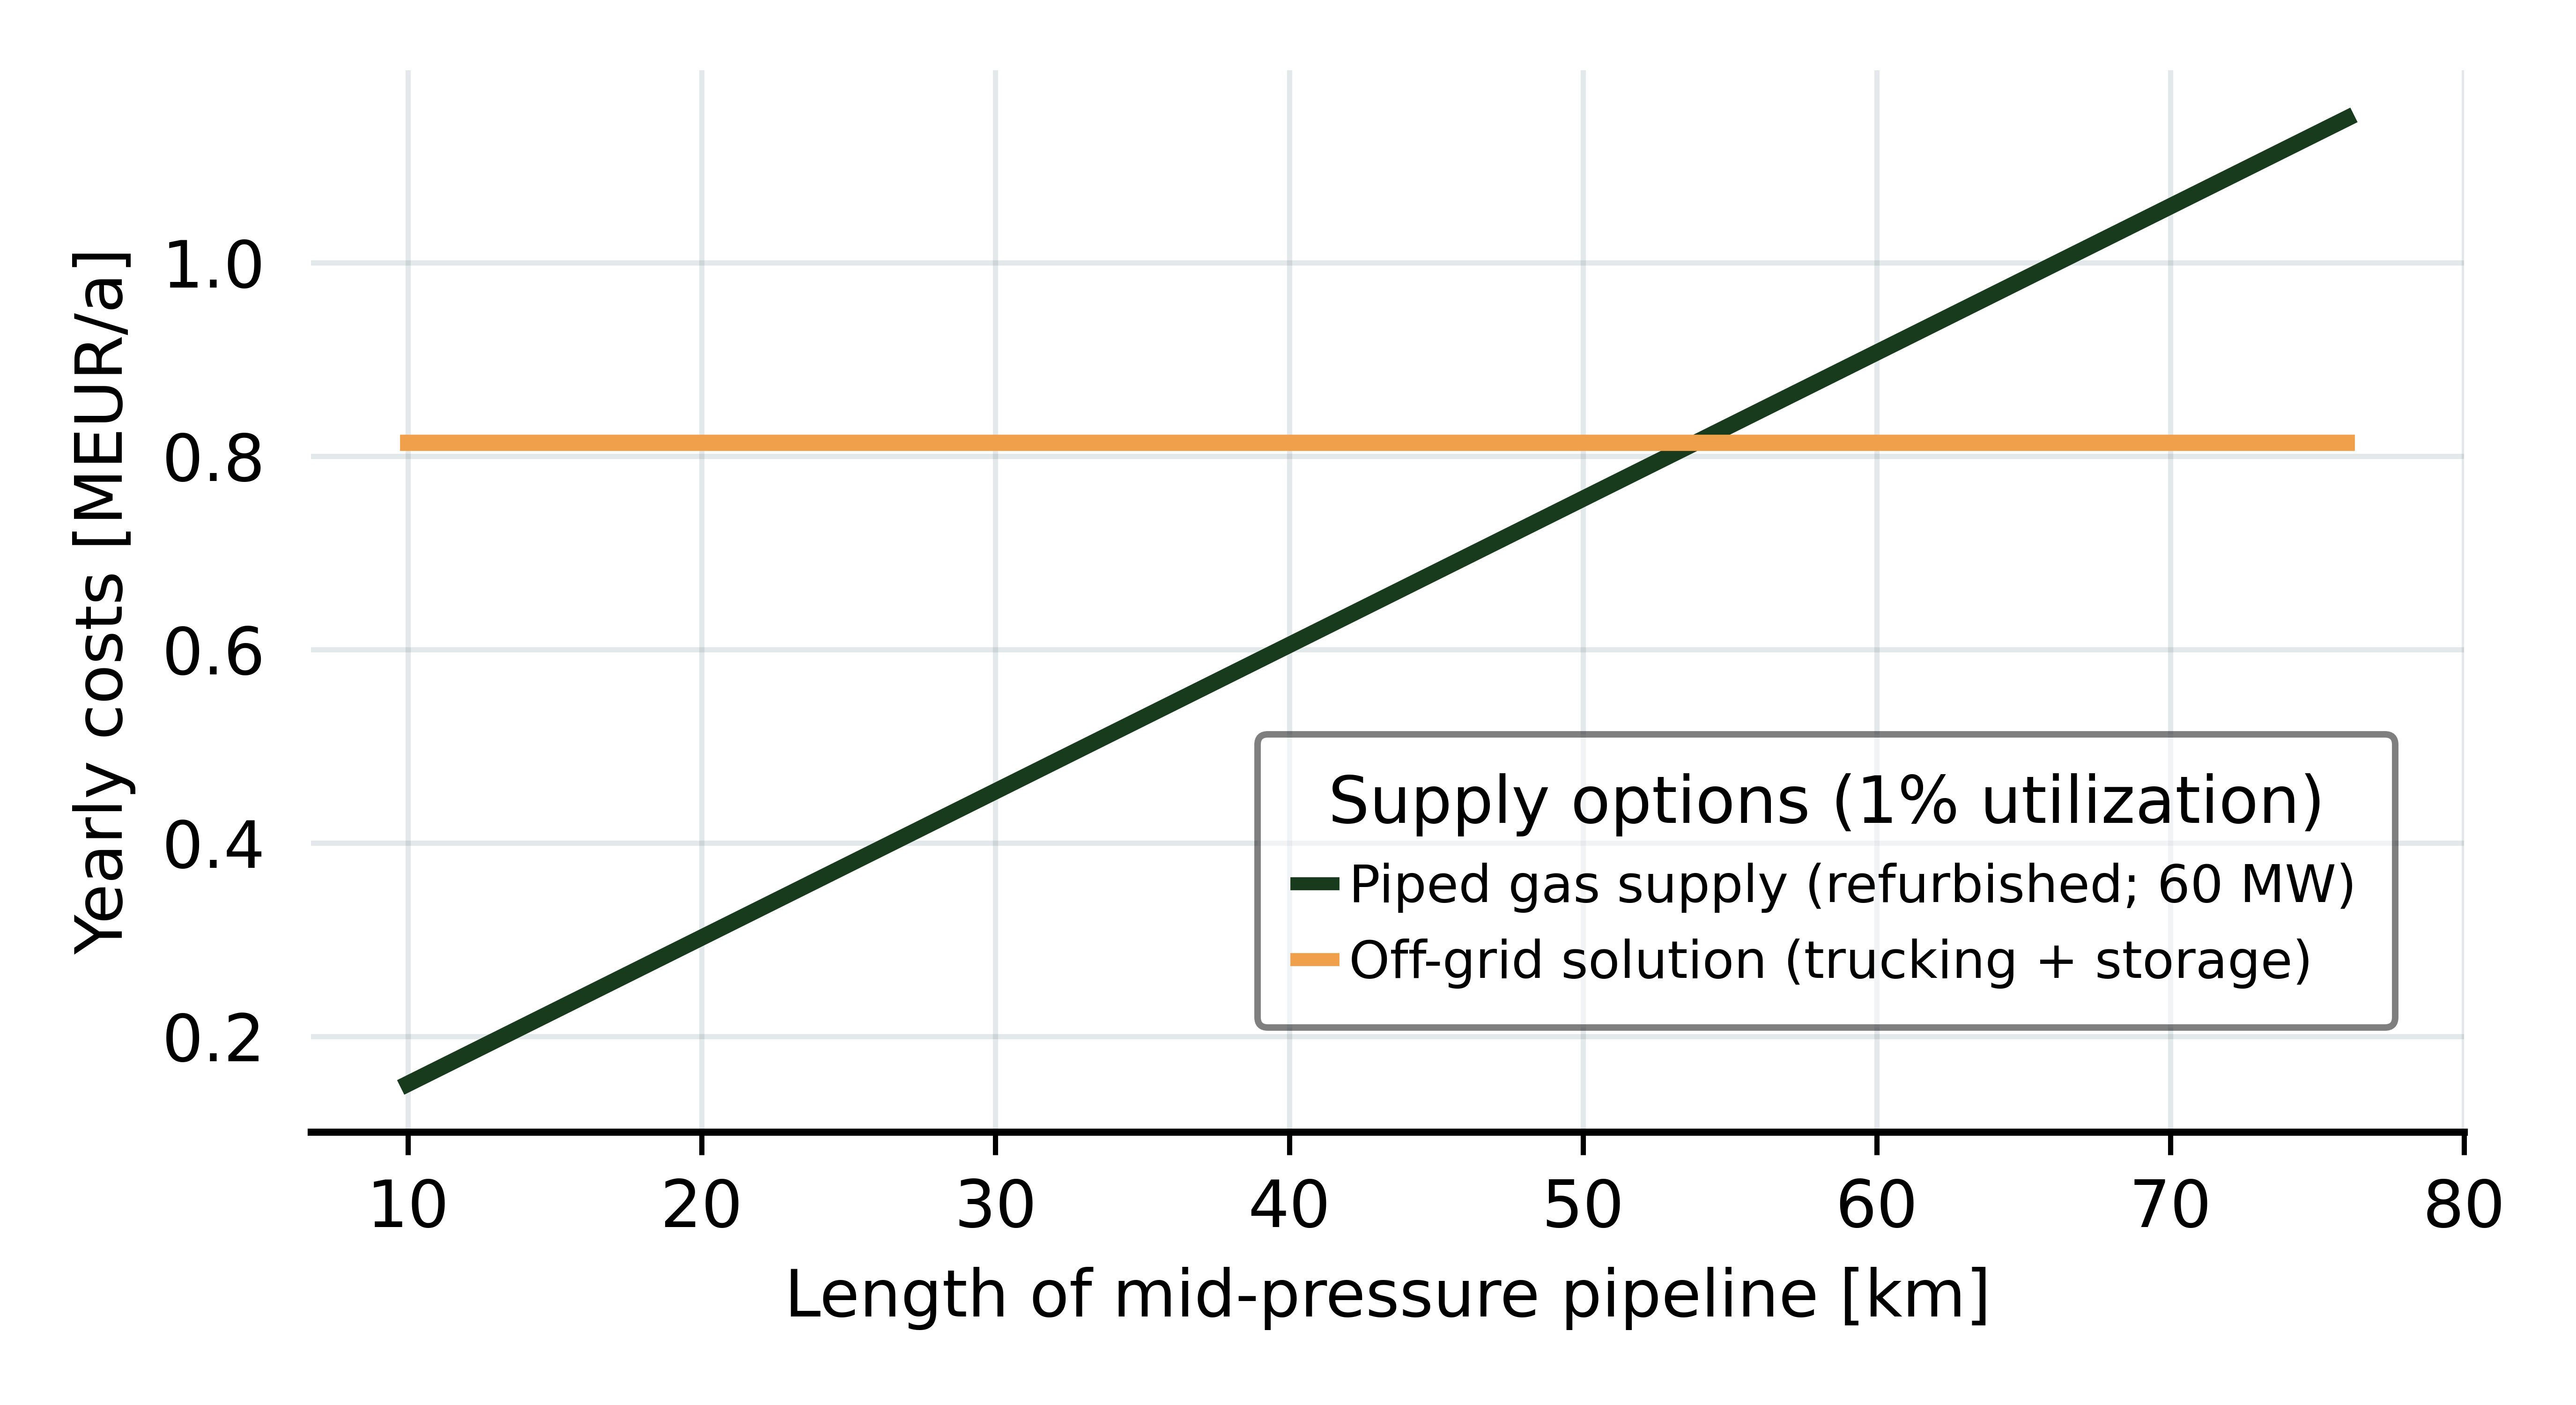
\includegraphics[width=1\linewidth]{figures/appendix/Illustration_Trade_Off_Auslastung.png}
	\caption{Illustration of the model's economic decision between piped gas supply and the off-grid solution. The amount of gas transported corresponds to \SI{1}{\%} of the total transport capacity (determined by an operation of the pipeline at its maximum capacity for the entire year).}
	\label{line_and_point}
\end{figure}





%
%\begin{sidewaystable}
%	\centering
%	\setlength{\extrarowheight}{.5em}
%	\resizebox{1\textwidth}{!}{
%		\begin{tabular}{cclll}
%			\toprule
%			\multicolumn{2}{c}{Equation} & \multicolumn{3}{c}{Qualitative/high-level explanation of the mathematical formulation}\\\cmidrule(lr){1-2}\cmidrule(lr){3-5}
%			Number & Dimension & Type & Keyword & Description\\\hline
%			\ref{objective} & 1 & Economic & Objective &  Minimize gas network operator's total costs\\
%			\ref{eq:capex} & 1 & Economic  & Capex &  Capital cost of the gas pipelines\\
%			\ref{eq:opex} & 1 & Economic & Opex & Fixed operating costs of gas pipelines\\
%			\ref{eq:total_book_value} & ($p \times l \times y$) & Economic & Book values & Book value per gas pipeline, network level and year\\
%			\ref{eq:revenues} & ($n \times l \times y \times m$) & Economic & Revenues & Revenues for supplying gas demand through network charge\\
%			\ref{bound1}, \ref{bound2} & ($p \times l \times y$) & Technical & Gas transport & Restriction of the gas transport per gas pipeline, network level and year\\
%			\ref{eq:balance} & ($n \times l \times y \times m$) & Technical & Gas balance & Gas balance constraint per node, network level, year and month\\
%			\ref{eq:demand} &  ($n \times l \times y \times m$) & Technical & Gas demand & Total gas demand as sum of local demand and delivered gas\\
% 			\ref{eq:source} &  ($n \times l \times y \times m$) & Technical & Gas source & Total gas source as sum of local production and gas delivered\\
%			\bottomrule
%	\end{tabular}}
%	\caption{\added{Overview of the model's mathematical formulation. Abbreviations: Gas pipeline (p), Network level (l), Node (n), Year (y), Month (m)}}
%	\label{tab:brief}
%\end{sidewaystable}


\end{document}